%% LyX 2.1.2.1 created this file.  For more info, see http://www.lyx.org/.
%% Do not edit unless you really know what you are doing.
\documentclass[10pt,english]{beamer}
\usepackage[T1]{fontenc}
\usepackage[latin9]{inputenc}
\usepackage{amsthm}
\usepackage{amsmath}
\usepackage{amssymb}

\DeclareMathOperator{\E}{\mathbb{E}}
\DeclareMathOperator*{\argmin}{arg\,min}

\makeatletter
%%%%%%%%%%%%%%%%%%%%%%%%%%%%%% Textclass specific LaTeX commands.
 % this default might be overridden by plain title style
 \newcommand\makebeamertitle{\frame{\maketitle}}%
 % (ERT) argument for the TOC
 \AtBeginDocument{%
   \let\origtableofcontents=\tableofcontents
   \def\tableofcontents{\@ifnextchar[{\origtableofcontents}{\gobbletableofcontents}}
   \def\gobbletableofcontents#1{\origtableofcontents}
 }

%%%%%%%%%%%%%%%%%%%%%%%%%%%%%% User specified LaTeX commands.
\usepackage{listings}
\usetheme{Warsaw}
% or ...
%\usetheme{Antibes}	% tree outline, neat
%\usetheme{JuanLesPins}	% like Antibes, with shading
%\usetheme{Bergen}	% outline on side
%\usetheme{Luebeck}	% like Warsaw, square sides
%\usetheme{Berkeley}	% interesting left bar outline
%\usetheme{Madrid}	% clean, nice.  7/12 page numbers
%\usetheme{Berlin}	% dots show slide number
%\usetheme{Malmoe}	% OK, plain, unshaded
%\usetheme{Boadilla}	% nice, white bg, no top bar
%\usetheme{Marburg}	% nice, outline on right
%\usetheme{boxes}	% ???
%\usetheme{Montpellier}	% tree outline on top, plainish white
%\usetheme{Copenhagen}	% like Warsaw
%\usetheme{PaloAlto}	% looks good
%\usetheme{Darmstadt}	% like Warsaw with circle outline
%\usetheme{Pittsburgh}
%\usetheme{default}
%\usetheme{Rochester}	% like boxy, unshaded warsaw
%\usetheme{Dresden}	% circle outline on top
%\usetheme{Singapore}	% purple gradient top
%\usetheme{Frankfurt}	% like Warsaw with circle outline on top
%\usetheme{Szeged}
%\usetheme{Goettingen}	% light purple right bar outline
%\usetheme{Warsaw}
%\usetheme{Hannover}	% like Goett with bar on left
%\usetheme{compatibility}
%\usetheme{Ilmenau}

\setbeamercovered{transparent}
% or whatever (possibly just delete it)

%\usecolortheme{seahorse}
%\usecolortheme{rose}

% seems to fix typewriter font in outline header:
\usepackage{ae,aecompl}

\makeatother

\usepackage{babel}

\title{Unlabeled data: Now it helps, now it doesn't}
\author{Mark Andrew Ward and Max Kuang}
\institute{Courant Institute}
\begin{document}


\pgfdeclareimage[height=0.5cm]{institution-logo}{institution-logo-filenameO}

\logo{\pgfuseimage{institution-logo}}

% RPD:  can't get this to work on any template.  not present in Warsaw any way, it seems

% hmm, problem seems to be that it isn't copied to the tmp dir, probably becuase it doesn't have the

% filename extension (which is tacked on by pgf it seems)

%\AtBeginSection[]{
\begin{frame}
\titlepage
\end{frame}
\AtBeginSubsection[]{

  \frame<beamer>{ 

    \frametitle{Outline}   

    \tableofcontents[currentsection,currentsubsection] 
%    \tableofcontents[currentsection] 

  }

}
%\beamerdefaultoverlayspecification{<+->}
\begin{frame}
     \frametitle{Outline}   
    \tableofcontents[currentsection,currentsubsection,sectionstyle = show,subsectionstyle = show] 
\end{frame}

\section{Introduction}
\subsection{Conflicting Views in Semi-supervised Learning}
\begin{frame}
\frametitle{\insertsubsection}
\begin{block}{Semi-supervised Learning}
 Given $n$ iid labeled samples $\{(x_i, y_i)\}_{i = 1,\dots, n}$ and $m$ iid unlabeled samples $\{x_i\}_{i = 1,\dots, m}$,
 semi-supervised learning attempts to make use of this combined information to surpass the learning performance
 that could be obtained by discarding the unlabeled data and doing supervised learning.
\end{block}

\begin{itemize}
 \item Not always helpful: Only when there exist a \textbf{link} between the \textbf{marginal data distribution $P(x)$} and the \textbf{target function to be learned $y = f(x)$}.
\item \textbf{Links}: \textbf{cluster assumption} and \textbf{manifold assumption}.
\end{itemize}


\end{frame}


\begin{frame}
 \frametitle{\insertsubsection}
\begin{itemize}
 \item Does unlabeled data help in error convergence rate under different assumptions?
\begin{center}
\begin{tabular}{l||ll}
 & SSL helps & SSL does not help\\ \hline\hline
Cluster assuption & Castelli, Cover & Rigollet\\
Manifold assuption & Lafferey and Wasserman & Niyogi
\end{tabular}
\end{center}
\end{itemize}
\end{frame}
\begin{frame}
\frametitle{\insertsubsection}
\begin{itemize}
\item
This work focuses on learning under the \textbf{cluster assumption} and provides \textbf{finite sample bounds} to identify situations in which unlabeled data will help to improve learning.
\end{itemize}
\begin{figure}[h]
\centering
 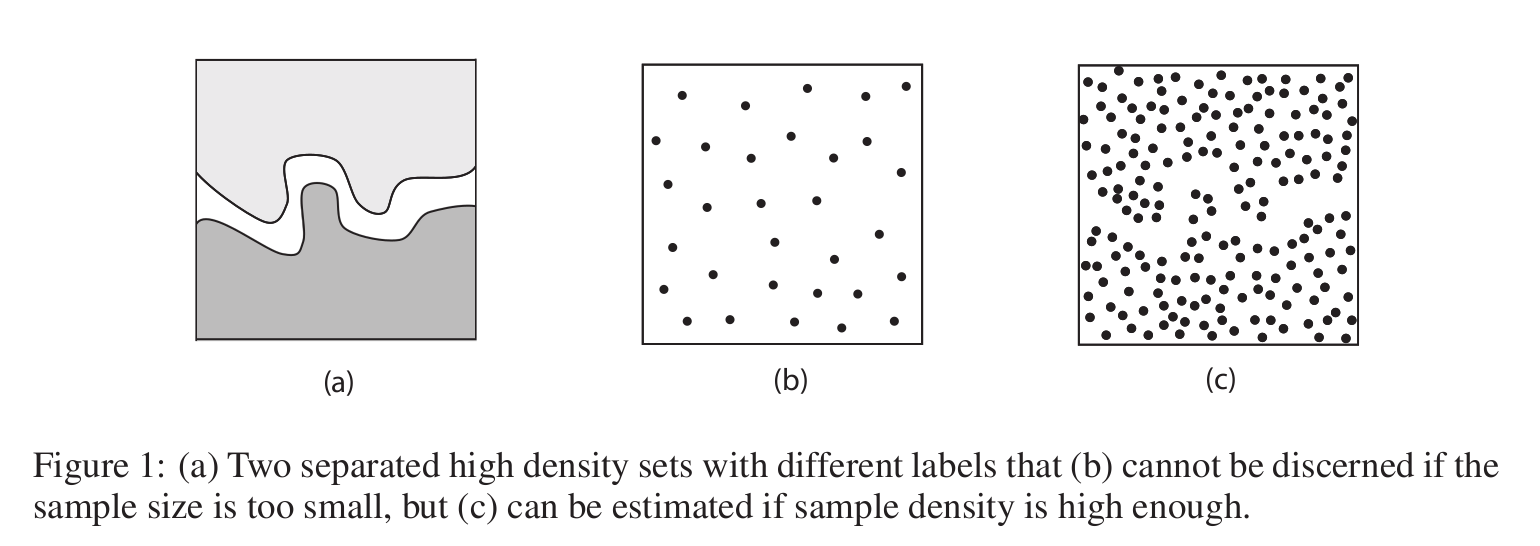
\includegraphics[width = 4in]{1.png}
\end{figure}
\end{frame}

\subsection{The Cluster Assumption}
\begin{frame}
 \frametitle{\insertsubsection: Marginal Distributions}
\begin{itemize}
\item The marginal distribution $p(x) = \sum_{k=1}^K a_k p_k(x)$ is the mixture of a finite, but unknown, number of component densities $\{p_k\}_{k=1}^K$.
\item Restrictions on $p_k$:
\begin{enumerate}
 \item $p_k$ is supported on a compact connected set $C_k\in\mathcal{X}$ with Lipschitz boundaries. Specifically:
\begin{equation}
\begin{array}{ll}
 C_k = \{&x\equiv (x_1,x_2,\dots,x_d)\in\mathcal{X}: 
\\&g_k^{(1)}(x_1,x_2,\dots,x_{d-1}) \leq x_d\leq  g_k^{(2)}(x_1,x_2,\dots,x_{d-1})\}
\end{array}
\end{equation}

\item $p_k$ is bounded from above and below, $0<b\leq p_k\leq B$.
\item $p_k$ is Holder-$\alpha$ smooth on $C_k$ with Holder constant $K_1$.
\end{enumerate}
\end{itemize}
\end{frame}
\begin{frame}
 \frametitle{\insertsubsection: Dicision Sets}
\begin{itemize}
 \item Let $\mathcal{D}$ denote the collection of all non-empty sets obtained as intersections of $\{C_k\}_{k=1}^K$.
 \item \textbf{Cluster assumption: the target function $y = f(x)$ to be learnt is smooth on each set $D\in\mathcal{D}$}.
\begin{figure}[h]
\centering
 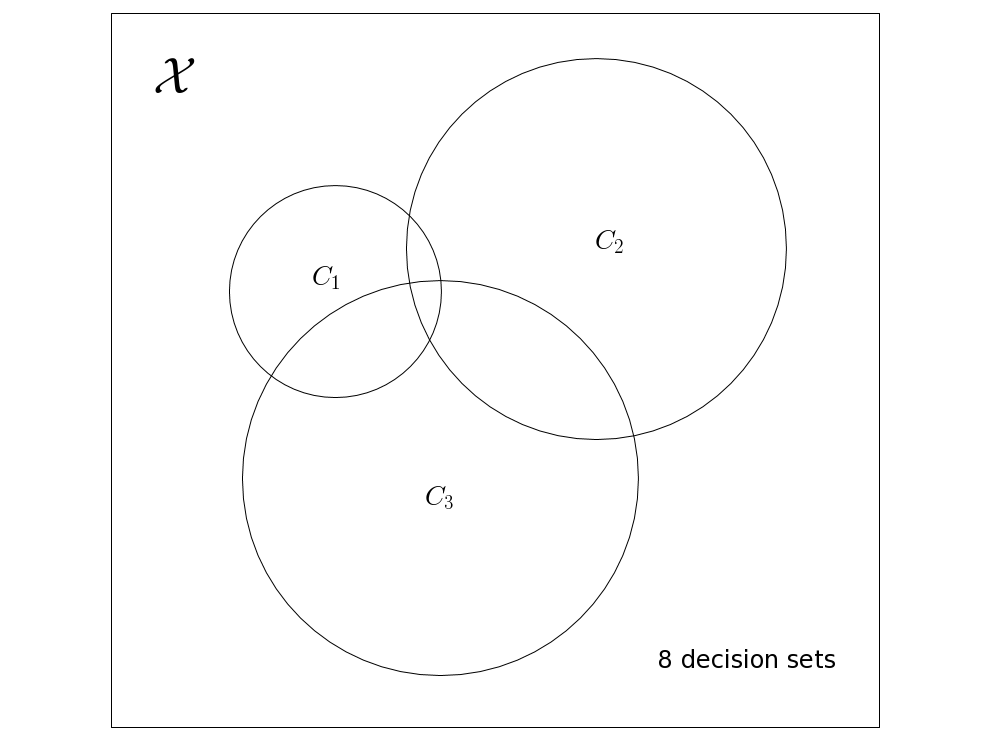
\includegraphics[width = 2.5in]{4.png}
\end{figure}
\end{itemize}
\end{frame}
\begin{frame}
\frametitle{\insertsubsection: Margin $\gamma$}
\begin{itemize}
 \item The margin $\gamma$ of a distribution is defined to be the minimal width of a decision set.
\item The margin $\gamma$ is assigned a positive sign if there is no overlap between components,otherwise it is assigned a negative sign.
\begin{figure}[h]
\centering
 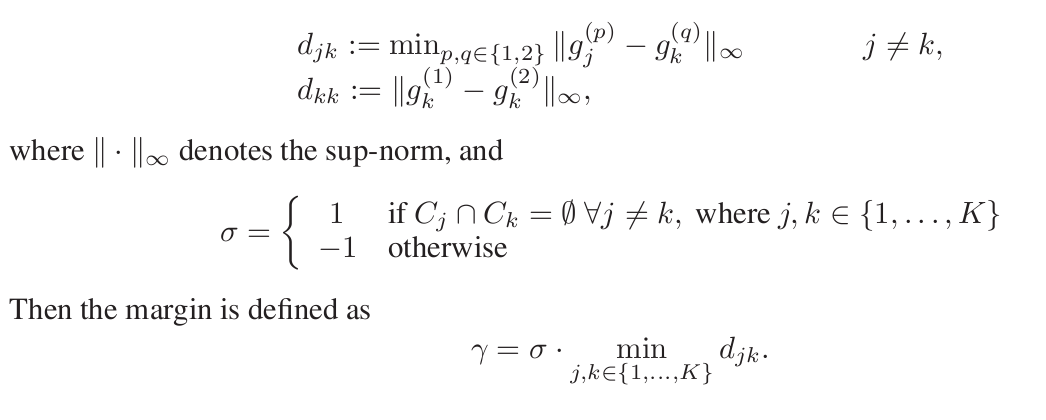
\includegraphics[width = 4in]{2.png}
\end{figure}
\end{itemize}
\end{frame}


\section{Finite Sample Analysis of Semi-supervised Learning}
\subsection{Summary}
\begin{frame}
 \frametitle{\insertsubsection}
\begin{itemize}
 \item Under cluster assumption, we are trying to figure out for what $(n,m,\gamma)$(and possibly other constraints) SSL surpasses SL
for all general learners.
\begin{center}
  \large    SSL > SL\\
$\Uparrow$\\
SSL Learner $\approx$ Clairvoyant Learner > General SL Learner
$\Uparrow$(definition)\\
\textit{Supervised learners with perfect knowledge of the decision sets $\mathcal{D}$}
 \end{center}
\end{itemize}

\end{frame}
\subsection{Learning the Decision Sets}
\begin{frame}
 \frametitle{\insertsubsection: \\SSL Learner $\approx$ Clairvoyant Learner}
\begin{itemize}
 \item Decision sets are learnable using unlabeled data: marginal density $p$ is smooth within each decision set but exhibits jumps at the decision set boundaries.
\item Main learning procedures:
\begin{enumerate}
 \item Marginal Density Estimation: From unlabeled sample $\{x_i\}_{i = 1,\dots, m}$ to density estimator $\hat{p}(x)$
\item Decision Set Estimation: From  $\hat{p}(x)$ to decision set estimator $\hat{\mathcal{D}}$
\end{enumerate}
\end{itemize}
\end{frame}
\begin{frame}
 \frametitle{\insertsubsection: Marginal Density Estimation}
\begin{itemize}
 \item Consider a uniform grid over the feature space $\mathcal{X} = [0,1]^d$ with spacing $2h_m$, where $h_m = \kappa_0 ((\log m)^2/m)^{1/d}$.
\item Make a histogram-style density estimation on the grid using kernel density estimation: 
\begin{equation}
 \hat{p}(x) = \frac{1}{mh_m^d}\sum_{i = 1}^m G(H^{-1}_m(X_i - \bar{x}))
\end{equation}
Where $\bar{x}$ is the closest point to $x$ on the grid, $G$ is the kernel and $H_m = h_mI$
\begin{figure}[h]
\centering
 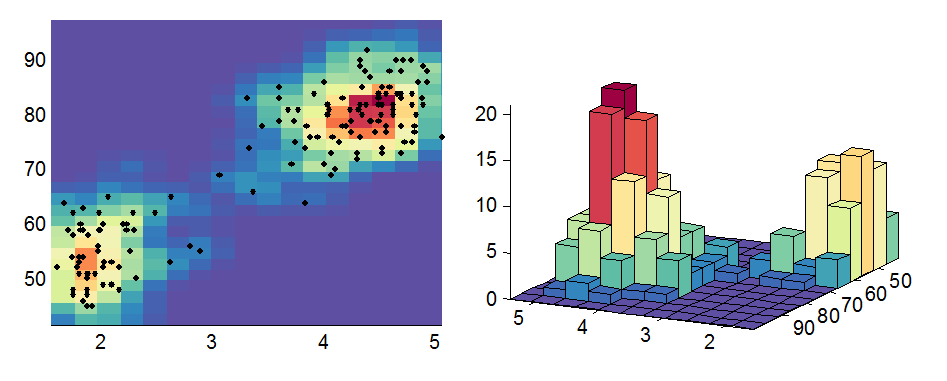
\includegraphics[width = 3in]{5.png}
\end{figure}
\end{itemize}
\end{frame}
\begin{frame}
 \frametitle{\insertsubsection: Decision Set Estimation}
\begin{itemize}
 \item Locating the jumps in $\hat{p}(x)$: \textbf{p-connectivity} of data points.
\item Two point $x_1,x_2\in \mathcal{X}$ are said to be \textbf{connected},
if there exists a sequence of points $x_1 = z_1 , z_2 ,\dots, z_l= x_2$ such that $z_2 , . . . , z_{l-1} \in U$,$\|z_j - z_{j+1}\leq 2\sqrt{d}h_m\|$.
\item Two point $x_1,x_2\in \mathcal{X}$ are said to be \textbf{p-connected}, if in addition to being \textbf{connected}, 
we have $|\hat{p}(z_i) - \hat{p}(z_j)| \leq (\log m)^{-1/3}$ for all $z_i, z_j$ satisfying $\|z_j - z_{j+1}\|\leq h_m\log m$.
\item All points that are pairwise \textbf{p-connected} specify an empirical decision set $\hat{D}$ and we derived $\hat{\mathcal{D}}$.
\end{itemize}
\end{frame}
\begin{frame}
 \frametitle{\insertsubsection: Guarantee}
\begin{figure}[h]
\centering
 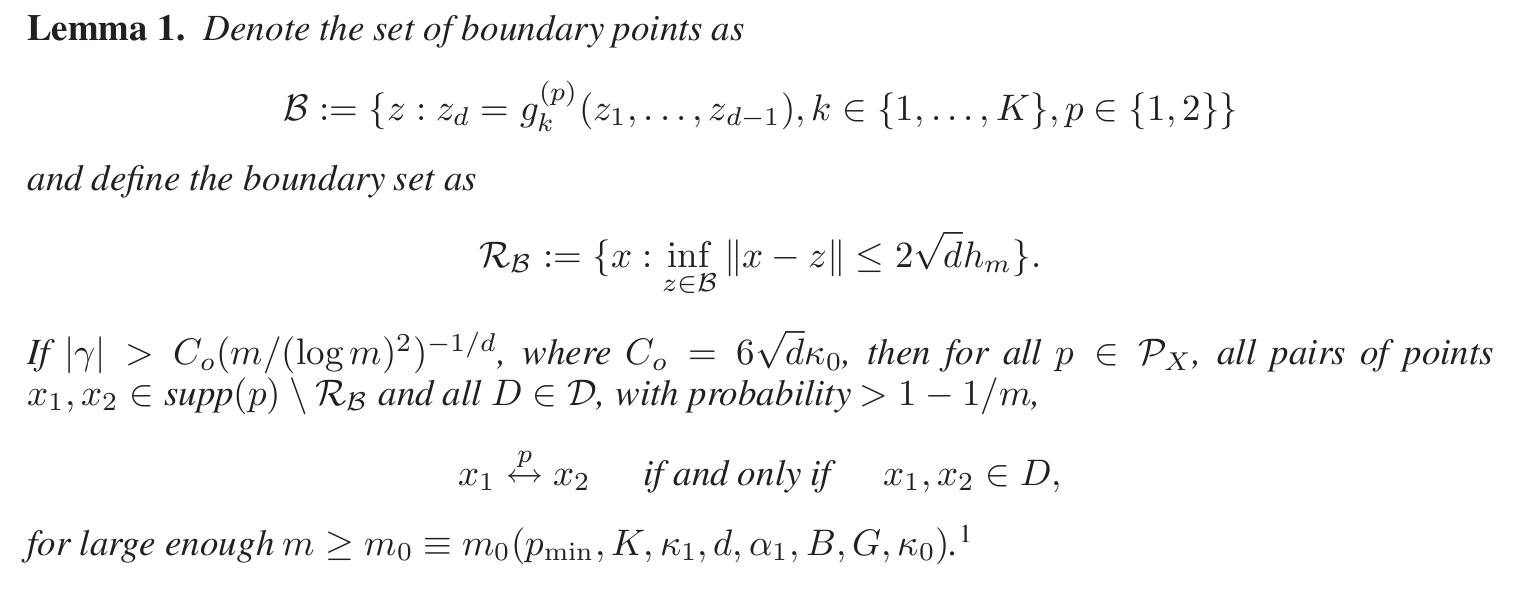
\includegraphics[width = 4in]{6.png}
\end{figure}
\begin{itemize}
 \item Exclude decision boundaries, p-connectivity is equivalent to decision set with high probability.
\item Margin $\gamma$ plays an important role: theorem works only when $|\gamma|$ is in the order of the spacing $h_m$.
\end{itemize}
\end{frame}
\begin{frame}
 \frametitle{\insertsubsection: Proof}
 \begin{enumerate}
  \item Uniform bound for density estimation: Given certain assumptions on Kernels, we have
  with probability at least $1 - \frac{1}{m}$:
  \begin{equation}
   \sup_{x\in supp(p)\backslash\mathcal{R_B}}|p(x) - \hat{p}(x)| < \bigg|h_m^{\min(1,\alpha_1)}+ \sqrt{\frac{\log m}{m _m^d}}\bigg|
  \end{equation}

  \item Conectivity: For all $x\in supp(p)\backslash\mathcal{R_B}$, with probability $1-\frac{1}{m}$, there exsits an unlabeled sample $X_i$ that
  $\|X_i - x\|< \sqrt{d}h_m$

  \item Bound $|\hat{p}(x) - \hat{p}(x')|$ using nearby unlabeled points $z,z'$:
$|\hat{p}(x) - \hat{p}(z)|$,$|\hat{p}(z) - \hat{p}(z')|$, $|\hat{p}(z) - p(z)|$ and $|p(z) - p(z')|$
 \end{enumerate}


\end{frame}

\subsection{SSL Performance Analysis}
\begin{frame}
 \frametitle{\insertsubsection}
 \begin{itemize}
  \item Let $\mathcal{R}(f)$ denote the risk of interest for a given target function $f$ and excess risk $\mathcal{E}(f) = \mathcal{R}(f) - \mathcal{R^*}$,
  where $\mathcal{R^*}$ is the infimum risk over all possible learners.
  \item SSL learner$\approx$ clairvoyant learner:
 \end{itemize}

 \begin{figure}[h]
\centering
 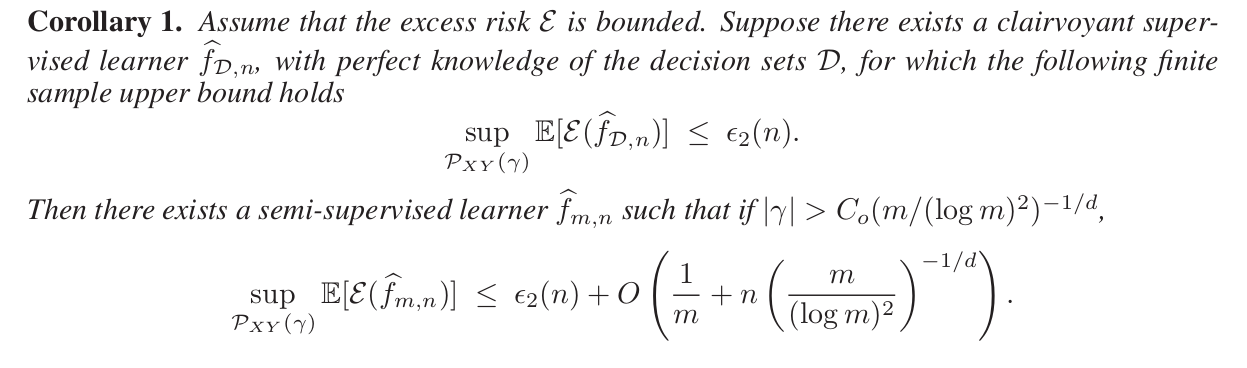
\includegraphics[width = 4.3in]{7.png}
\end{figure}
\end{frame}
\begin{frame}
 \frametitle{\insertsubsection: Proof and Remarks}
 \begin{itemize}
  \item To prove the theorem, one only need to use the fact that $\hat{\mathcal{D}}$ is very close to $\mathcal{D}$
  in a probability sense. Using condition probability, $\E \mathcal{E}(\hat{f}_{m,n})$ is close to $\E \mathcal{E}(\hat{f}_{D,n})$.
  \item Conditions to make SSL Learner be close to clairvoyant learner are:
  \begin{enumerate}
   \item The margin $\gamma$ is large enough: $|\gamma| > C_0(m/(\log m)^2)^{-1/d} $
   \item The error term is smaller than $\varepsilon_2(n)$: $(n/\varepsilon_2(n))^d = O(m/(\log m)^2)$
  \end{enumerate}
  \item If the clairvoyant learner outperforms general SL learners: 
  \begin{equation}
   \inf_{f_n}\sup_{P_{XY}}\E[\mathcal{E}(f_n)] \geq \varepsilon_1(n) > \varepsilon_2(n)
  \end{equation}
  We have that there exists a SSL Learner that outperforms general SL learners.
 \end{itemize}

\end{frame}

\section{Density-adaptive Regression}
\subsection{Optimal Decision Rule}
\begin{frame}
   \frametitle{\insertsubsection: Definition}
  \begin{itemize}
	\item $Y$ continuous and bounded random variable
	\item $f^*(x)=\E[Y|X=X]$, under the squared error loss
	\item Let $\E_k$ denote expectation with respect to $p_k(Y|X=x)$ and define $f_k(x) = \E_k[Y|X=x]$ then 
	\begin{equation}
	f^* (x) = \sum_{k=1}^{K} \frac{\sum_{j=1}^{K} a_k p_k(x)} {a_j p_j(x)} f_k(x)
	\end{equation}
	\item Assumptions: 
	\begin{enumerate}
	\item $f_k$ is uniformly bounded, $|f_k| \leq M$
	\item $f_k$ is Holder-$\alpha$ smooth on $C_k$
	\end{enumerate}
   \end{itemize} 
\end{frame}

\subsection{SSL Algorithm}
\begin{frame}
   \frametitle{\insertsubsection}
   \begin{itemize}
     \item Since $f^*$ is smooth on each $D \in \mathcal{D}$, perform local polynomial fits within each empirical decision set, using labeled training data that are p-connected
     \item Use spatially adaptive estimator, optimal for piecewise-smooth functions
     \item Guarantee SSL still achieves an error bound that is no worse than lower bound for SL when components are indiscernible even with unlabeled data.
   \end{itemize}
\end{frame}
\begin{frame}
   \frametitle{\insertsubsection}
   \begin{itemize}
   \item Semi-supervised learner: 
   \begin{align}
     \hat{f}_{m,n,x}(\cdot) &= \argmin_{f^{'} \in \Gamma} \sum_{i=1}^{n} (Y_i - f'(X_i) )^2 \mathbf{1}_{x \overset{p}\longleftrightarrow X_i} + \text{pen}(f') \\
     \hat{f}_{m,n}(x) &\equiv  \hat{f}_{m,n,x}(\cdot) \notag
   \end{align}
   \item $\Gamma$: collection of piecewise polynomials, defined over a partitioning of the domain $\mathcal{X} = [0,1]^d$
   \item pen($f'$) $\propto$ $log(\sum_{i=1}^{n}\mathbf{1}_{x \overset{p}\longleftrightarrow X_i}) \cdot \text{\#} f'$, where \#$f'$ is the number cells over which $f'$ is defined
   \end{itemize}
\end{frame}

\subsection{Error Bounds}
\begin{frame}
   \frametitle{\insertsubsection:  Overview}
   \begin{itemize}
   \item bounds
   \end{itemize}
\end{frame}
   
\end{document}


